\documentclass[18pt, 4paper]{article}
\usepackage[ngerman]{babel}
\usepackage[T1]{fontenc}

\usepackage[utf8]{inputenc}
\usepackage{setspace}
\usepackage{amsmath}
\usepackage{amsfonts}
\usepackage{verbatim}
\usepackage{fancyhdr}
\usepackage{graphicx}
\usepackage[left=2cm, top=2cm, right=2cm, bottom=1.5cm]{geometry}
\usepackage{graphicx}
\usepackage{sidecap}
%\usepackage{polynom}
%\usepackage[yyyymmdd]{datetime}
%\renewcommand{\dateseparator}{}
%\usepackage{datetime2}

%\polyset{style=C}
\pagestyle{fancy} %eigener Seitenstil
\fancyhf{} %alle Kopf- und Fußzeilenfelder bereinigen
\fancyhead[L]{Differenzialrechnung-Funktionen} %Kopfzeile links
\fancyhead[C]{Fabian Pfaff} %zentrierte Kopfzeile
\fancyhead[R]{\today} %Kopfzeile rechts
\fancyfoot[L]{Differenzialrechnung-Funktionen} %Fußzeile links
\fancyhead[C]{Fabian Pfaff} %zentrierte Kopfzeile
\fancyfoot[C]{\thepage} %Seitennummer
\fancyfoot[R]{\today}
\renewcommand{\footrulewidth}{0.4pt} %untere Trennlinie

\begin{document}
\section*{Aufgabe1}
Bestimmen Sie jeweils die Definitionsmenge D, die Wertemenge W, die Gleichung $y=f^{-1}(x)$ der Umkehrfunktion $f^{-1}$. Prüfen Sie, ob $f^{-1} \circ f$ die identische Funktion auf $D_f$ und $f \circ f^{-1}$ die identische Funktion auf $W_f$ ist

\subsection*{b)}
$f(x)=\frac{1-x}{2x+1}$\\
\\
$D_f = \mathbb{R}\setminus\{\frac{1}{2}\}$\\
\\
$W_f = \mathbb{R}$
\subsubsection*{Berechnung der Inversen}
\begin{flalign*}
	y&=\frac{1-x}{2x+1} &|\cdot(2x+1) &&&\\
	2xy+y &= 1-x &|+x-y &&&\\
	2xy+x &= 1-y &&&&\\
	x(2y+1) &= 1-y &|\div(2y+1) && &\\
	x &= \frac{1-y}{2y+1}&&&&\\
	\Rightarrow f^{-1}=f\\
\end{flalign*}
\subsubsection*{Überprüfung der Inversen}
Da $f$ seine eigene Inverse ist muss nur eine Richtung überprüft werden.
%\[\polyfactorize{x^2+1}\]
%\[\polylongdiv{x^2-1}{x-1}\]
\begin{flalign*}
	f \circ f^{-1}&=\frac{1-\frac{1-x}{2x+1}}{2\left(\frac{1-x}{2x+1}\right)+1}\\
	&=\frac{\frac{2x+1-(1-x)}{2x+1}}{\frac{2-2x+2x+1}{2x+1}}\\
	&=\frac{2x+1-(1-x)}{2-2x+2x+1}\\
	&=\frac{3x}{3}\\
	f \circ f^{-1}&=x
\end{flalign*}
Der Graph der Funktionen befindet sich im Anhang
\newpage

\subsection*{c)}
$f(x)=\ln(x+2)$\\
\\
$D_f = (-2,\infty)$\\
\\
$W_f = \mathbb{R}$
\subsubsection*{Berechnung der Inversen}
\begin{flalign*}
	y=\ln(x+2)\quad	&| e^{(\cdots)} \\
	e^y =x+2\quad	&| -2 \\
	x=e^y-2\\
	\Rightarrow f^{-1}=e^x -2\\
\end{flalign*}
\subsubsection*{Überprüfung der Inversen}
\begin{flalign*}
	f \circ f^{-1}	&=\ln(e^x -2 +2)\\
			&=\ln(e^x)\\
	f \circ f^{-1}	&=x\\
	&\\
	f^{-1} \circ f	&=e^{\ln(x+2)}-2\\
			&=x+2-2\\
	f^{-1} \circ f	&=x
\end{flalign*}
Der Graph der Funktionen befindet sich im Anhang
\subsection*{d)}
$f(x)=\cos(x)$\\
\\
$D_f = (-\infty,\infty)$\\
\\
$W_f = [-1,1]$
\subsubsection*{Berechnung der Inversen}
Die Cosiunusfunktion kann nicht auf seinem kompletten Definitionsbereich invertiert werden. Da mehrere x-Werte den selben Funktionswert ergeben. Damit man eine Umkehrfunktion bilden kann muss der Definitionsbereich eingeschränkt werden, sodass jeder erhaltene Funktionswert eindeutig ist. Man schränkt hierfür den Wertebereich auf $[0,  \pi]$ ein. In diesem Bereich kann eine Umkehrfunktion gebildet werden. Der vorher gennante Wertebereich ändert sich dabei nicht.

Der Graph der Funktionen befindet sich am Ende des Dokumentes
\newpage
\begin{figure}
	\centering
	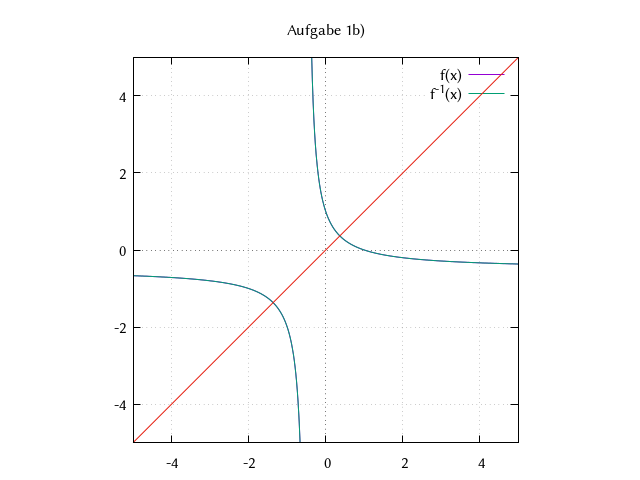
\includegraphics[scale=0.4]{images/Aufgabe2.png}
	\caption{Graph der Funktion $f(x)=\frac{1-x}{2x+1}$ und seiner Inversen. Da beide 			Funktionen identisch sind überlagern sich die Farbe}
	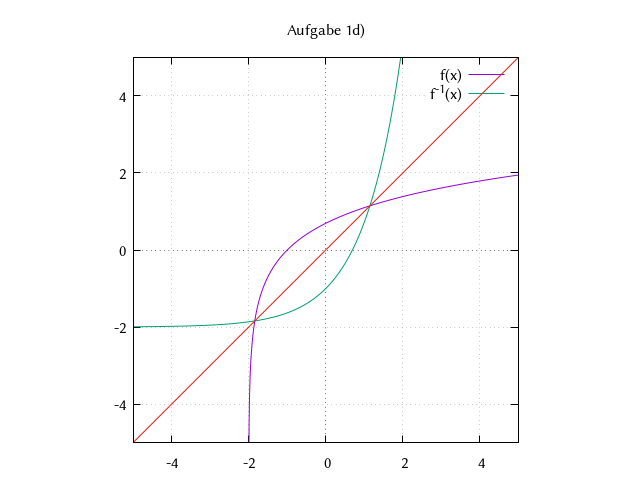
\includegraphics[scale=0.4]{images/Aufgabe3.png}
	\caption{Graph der Funktion $f(x)=\ln(x+2)$ und seiner Inversen.}
	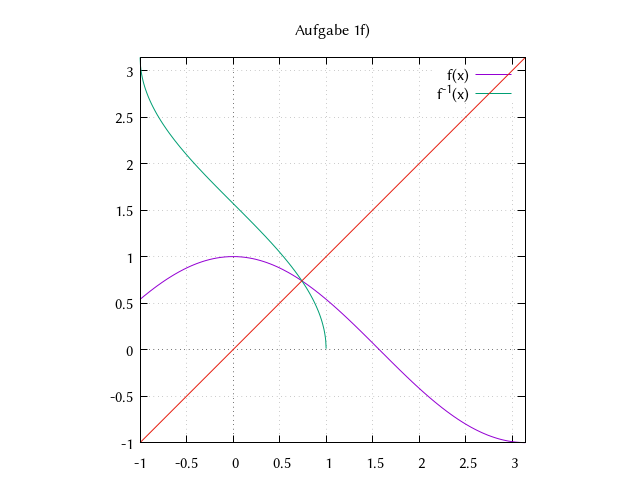
\includegraphics[scale=0.4]{images/Aufgabe4.png}
	\caption{Graph der Funktion $\cos(x)$ und seiner Inversen. Die Umkehrung f				indet nur im Bereich $x= [0:\pi]$ statt}
\end{figure}
\end{document}

